\documentclass[11pt]{article}

% Bioinformatics Application Note style packages
\usepackage[utf8]{inputenc}
\usepackage[T1]{fontenc}
\usepackage{geometry}
\geometry{a4paper, margin=2.5cm}
\usepackage{authblk}
\usepackage{graphicx}
\usepackage{booktabs}
\usepackage{multirow}
\usepackage{hyperref}
\usepackage{xcolor}
\usepackage{listings}
\usepackage{natbib}
\usepackage{amsmath}
\usepackage{microtype}
\usepackage{float}
\usepackage{subcaption}

% Code listing style
\lstset{
    basicstyle=\ttfamily\small,
    breaklines=true,
    frame=single,
    backgroundcolor=\color{gray!10},
    keywordstyle=\color{blue},
    commentstyle=\color{green!50!black},
    stringstyle=\color{red!60!black}
}

% Hyperlink colors
\hypersetup{
    colorlinks=true,
    linkcolor=blue!70!black,
    citecolor=blue!70!black,
    urlcolor=blue!70!black
}

\title{\textbf{hvantk: a Hail-based toolkit for scalable variant annotation, multi-omics integration, and downstream enrichment analysis}}

\author[1]{Enrique Audain}
\author[2]{Yasset Perez-Riverol}
\author[1]{Marc-Phillip Hitz}
\affil[1]{Department of Congenital Heart Disease and Pediatric Cardiology, University Hospital Schleswig-Holstein, Kiel, Germany}
\affil[2]{European Molecular Biology Laboratory, European Bioinformatics Institute (EMBL-EBI), Wellcome Genome Campus, Hinxton, Cambridge, UK}

\date{}

\begin{document}

\maketitle

%============================================================================
% ABSTRACT
%============================================================================
\begin{abstract}
\noindent\textbf{Summary:} The interpretation of genetic variants in large-scale sequencing studies requires integrating evidence across multiple omics layers and performing specialized downstream analyses. We present \textbf{hvantk} (Hail-based Variant Annotation Toolkit), a scalable Python toolkit built on the Hail framework that provides three key capabilities: (i) a unified multi-omics annotation framework integrating genomic (ClinVar, dbNSFP, gnomAD), transcriptomic (GTEx, Expression Atlas, UCSC Cell Browser), and proteomic (CPTAC, INSIDER) data sources; (ii) prediction score ROC analysis (PSROC) for systematic evaluation of variant pathogenicity classifiers; and (iii) gene set enrichment analysis (EnrichEx) supporting overlap enrichment and rare variant burden testing. hvantk seamlessly integrates with the Variant Dataset (VDS) format \citep{king2024svcr}, enabling scalable processing from single samples to population-scale cohorts. Additionally, the toolkit provides quality control computation and interactive HTML report generation. By combining scalable variant annotation with multi-omics integration and downstream enrichment analysis within a unified Hail-native framework, hvantk enables researchers to move efficiently from variant calls to biological insights.

\vspace{0.5em}
\noindent\textbf{Availability and Implementation:} hvantk is freely available under the Apache 2.0 license at \url{https://github.com/Clinical-Genomics-Lund/hvantk}. Documentation and tutorials are available at \url{https://hvantk.readthedocs.io}.

\vspace{0.5em}
\noindent\textbf{Contact:} enrique.audain@uksh.de

\vspace{0.5em}
\noindent\textbf{Supplementary information:} Supplementary data are available at \textit{Bioinformatics} online.
\end{abstract}

%============================================================================
% INTRODUCTION
%============================================================================
\section{Introduction}

The widespread adoption of next-generation sequencing in clinical and research settings has created an unprecedented demand for computational tools capable of annotating and interpreting genetic variants at scale \citep{karczewski2020mutational}. Modern variant interpretation increasingly demands a multi-omics perspective, integrating evidence from genomic annotations (pathogenicity predictions, population frequencies, clinical classifications), transcriptomic data (tissue and cell-type expression patterns), and proteomic information (protein expression levels, interaction networks) \citep{ritchie2015methods}. Furthermore, researchers need tools to evaluate variant pathogenicity prediction scores against clinical benchmarks and to test whether variants in functionally related gene sets are associated with phenotypes of interest.

Several challenges complicate this integration. First, annotation data are distributed across numerous public resources with heterogeneous formats, including ClinVar for clinical significance \citep{landrum2018clinvar}, dbNSFP for computational predictions \citep{liu2020dbnsfp}, gnomAD for population frequencies \citep{karczewski2020mutational}, and GTEx for tissue expression \citep{gtex2020gtex}. Second, existing annotation tools such as ANNOVAR \citep{wang2010annovar} and VEP \citep{mclaren2016ensembl} lack native support for multi-omics data integration and distributed computing at population scale. Third, downstream analyses such as gene set enrichment and burden testing often require custom scripting to interface with scalable genomic workflows.

Hail (\url{https://hail.is}) provides a powerful framework for scalable genomic analysis, and the recent introduction of the Variant Dataset (VDS) format has enabled efficient storage and manipulation of genetic data from cohorts with hundreds of thousands to millions of individuals \citep{king2024svcr}. However, translating variant data into biological insights requires additional analytical layers beyond what the core Hail framework provides.

Here, we present \textbf{hvantk} (Hail-based Variant Annotation Toolkit), a scalable toolkit that addresses these challenges through three complementary capabilities: (i) a unified framework for annotating variants and genes with data spanning genomic, transcriptomic, and proteomic layers; (ii) systematic evaluation of pathogenicity prediction scores (PSROC); and (iii) gene set enrichment analysis including rare variant burden testing (EnrichEx). By building natively on Hail, hvantk enables researchers to leverage distributed computing for large-scale analyses while providing the analytical depth required for comprehensive variant interpretation.

%============================================================================
% IMPLEMENTATION
%============================================================================
\section{Implementation}

hvantk is implemented in Python ($\geq$3.10) and built on the Hail framework (v0.2.137), leveraging its distributed data structures (Table, MatrixTable, VariantDataSet) for scalable genomic data processing. The toolkit follows a modular architecture with three core components (Figure~\ref{fig:workflow}).

\begin{figure}[t]
\centering
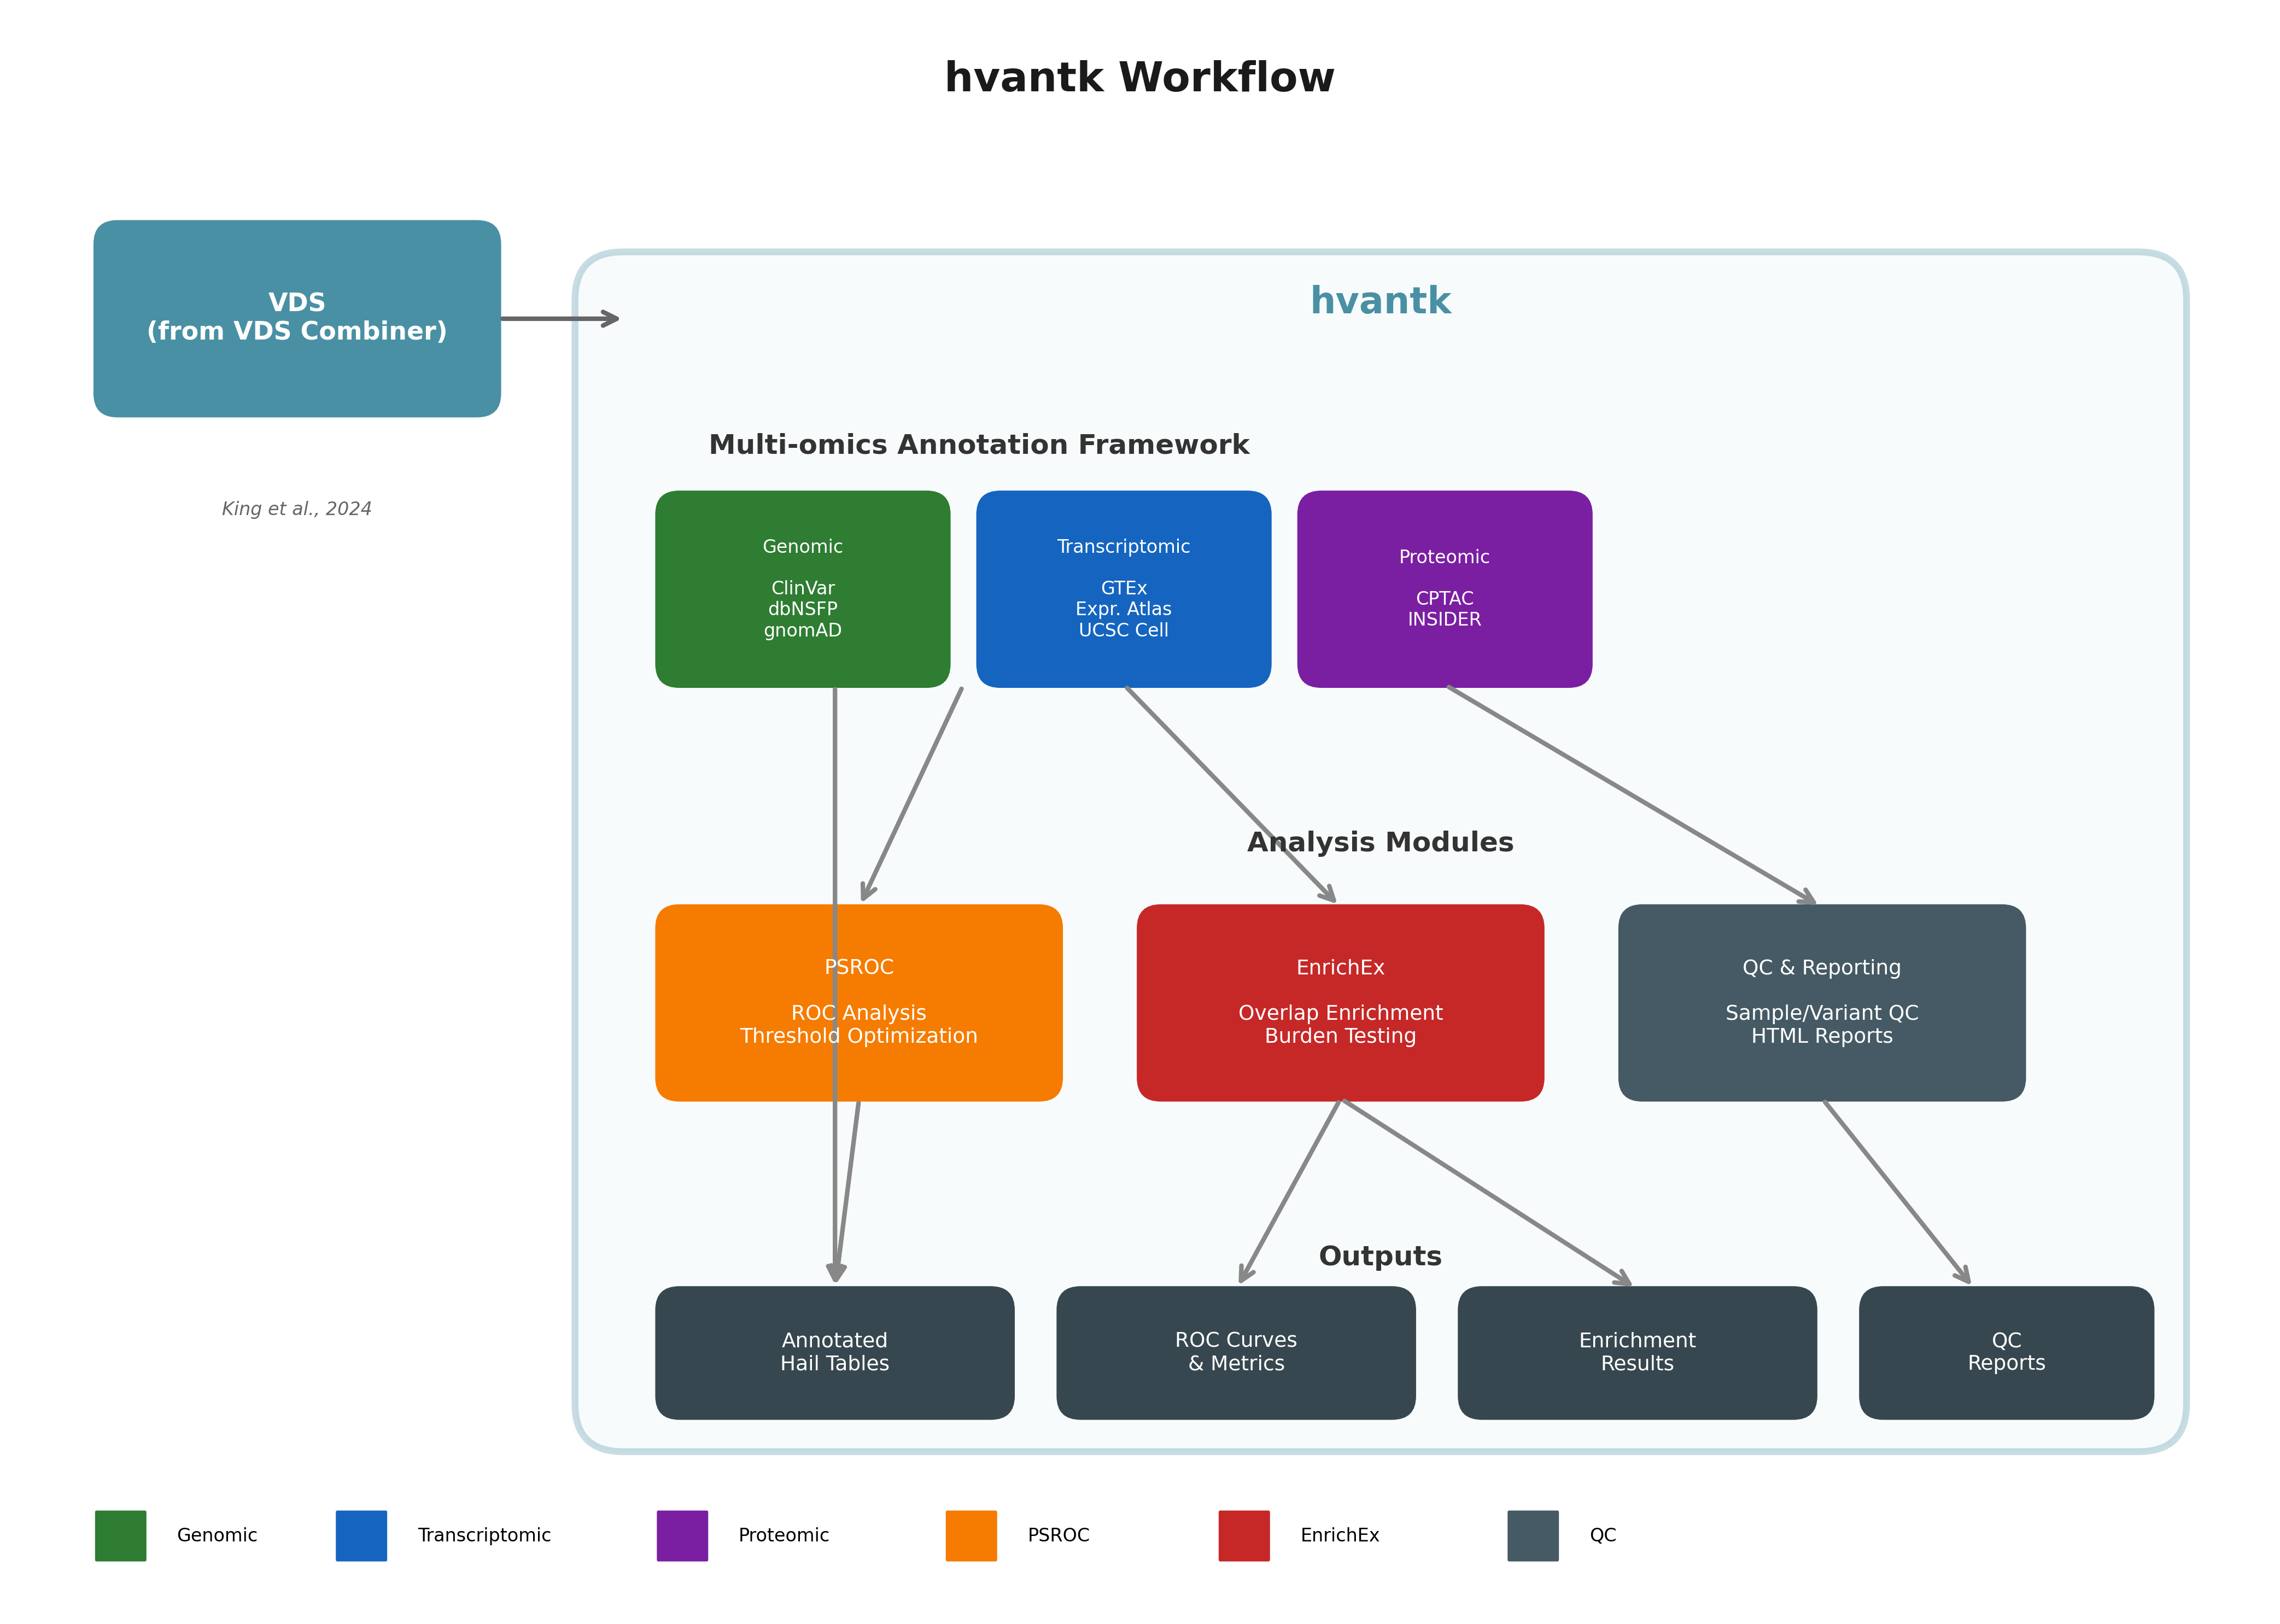
\includegraphics[width=\textwidth]{figures/fig1_workflow.png}
\caption{\textbf{hvantk workflow overview.} The toolkit provides three integrated components built on the Hail framework: (1) a multi-omics annotation framework integrating genomic, transcriptomic, and proteomic data sources; (2) analysis modules for prediction score evaluation (PSROC), gene set enrichment (EnrichEx), and quality control reporting; and (3) standardized outputs including annotated Hail Tables, ROC analysis results, enrichment statistics, and interactive QC reports.}
\label{fig:workflow}
\end{figure}

\subsection{Multi-omics Annotation Framework}

A key limitation of raw variant data---even when efficiently stored in VDS format---is the absence of functional context. hvantk addresses this through a unified annotation framework that integrates data across three omics layers (Table~\ref{tab:datasources}):

\textbf{Genomic annotations} provide variant-level context including clinical significance from ClinVar \citep{landrum2018clinvar}, computational pathogenicity predictions from dbNSFP \citep{liu2020dbnsfp} (CADD, REVEL, MetaLR, and 30+ additional scores), population allele frequencies from gnomAD \citep{karczewski2020mutational}, and regional constraint from CCR. Gene-level annotations include evolutionary constraint metrics (pLI, LOEUF, missense Z-scores) and gene-disease validity classifications from ClinGen \citep{rehm2015clingen}.

\textbf{Transcriptomic annotations} contextualize variants with expression data: bulk RNA-seq from GTEx \citep{gtex2020gtex} (54 tissues) and Expression Atlas \citep{papatheodorou2020expression}, and single-cell RNA-seq from the UCSC Cell Browser (hundreds of datasets across organs and developmental stages).

\textbf{Proteomic annotations} add protein-level evidence including expression quantification from CPTAC \citep{mertins2016proteogenomics} and protein-protein interaction networks from INSIDER.

The framework uses a protocol-based architecture (\texttt{Builder}, \texttt{Streamer}, \texttt{Downloader}) that enables seamless addition of new data sources. All annotations are stored as Hail Tables with standardized schemas, enabling efficient joins with VDS-derived MatrixTables. Both GRCh37 and GRCh38 reference genomes are supported with automatic liftover.

\begin{table}[t]
\centering
\caption{Multi-omics data sources integrated in hvantk.}
\label{tab:datasources}
\begin{tabular}{@{}llll@{}}
\toprule
\textbf{Omics Layer} & \textbf{Source} & \textbf{Data Type} & \textbf{Key Annotations} \\
\midrule
\multirow{4}{*}{Genomic} & ClinVar & Variant & Clinical significance, review status \\
 & dbNSFP & Variant & CADD, REVEL, MetaLR, 30+ scores \\
 & gnomAD & Variant & Population allele frequencies \\
 & ClinGen & Gene & Gene-disease validity \\
\midrule
\multirow{3}{*}{Transcriptomic} & GTEx & Bulk RNA-seq & TPM across 54 tissues \\
 & Expression Atlas & Bulk RNA-seq & Condition-specific expression \\
 & UCSC Cell Browser & scRNA-seq & Cell-type expression profiles \\
\midrule
\multirow{2}{*}{Proteomic} & CPTAC & Proteomics & Protein abundance \\
 & INSIDER & PPI & Protein-protein interactions \\
\bottomrule
\end{tabular}
\end{table}

\subsection{Prediction Score ROC Analysis (PSROC)}

Selecting appropriate pathogenicity prediction thresholds is critical for variant classification, yet systematic evaluation across genes and scores remains cumbersome. The PSROC module addresses this by computing ROC curves for user-specified prediction scores using ClinVar pathogenic/benign classifications as ground truth.

For each score, the module calculates the area under the ROC curve (AUC) and identifies optimal classification thresholds using three complementary methods: Youden's J statistic (maximizing sensitivity + specificity - 1), closest-to-corner (minimizing Euclidean distance to perfect classification), and F1-score optimization. The module also reports missingness rates, enabling informed decisions when scores are unavailable for substantial variant fractions. In our evaluation using variants from BRCA1, BRCA2, and TP53, REVEL achieved the highest discriminative performance (AUC = 0.998), followed by CADD (AUC = 0.979) and MetaLR (AUC = 0.896) (Supplementary Figure S1--S2, Table S1).

\subsection{Gene Set Enrichment Analysis (EnrichEx)}

The EnrichEx module provides two approaches for testing associations between variants and predefined gene sets:

\textbf{Overlap enrichment} uses Fisher's exact test to assess whether a query gene list (e.g., genes harboring rare variants in cases) is significantly enriched in biological pathways or disease-associated gene sets. Odds ratios with 95\% confidence intervals are computed, with Bonferroni or Benjamini-Hochberg correction for multiple testing (Supplementary Figure S3, Table S2).

\textbf{Burden testing} leverages Hail's regression framework to test whether rare variant burden in gene sets differs between cases and controls (logistic regression) or correlates with quantitative traits (linear regression). Variants can be filtered by allele frequency, VEP consequence, and pathogenicity score thresholds (e.g., CADD $>$ 20). Covariate adjustment for population structure and demographic variables is supported (Supplementary Figure S4, Table S3).

\subsection{Quality Control and Reporting}

While the VDS Combiner efficiently combines GVCFs, downstream analysis requires quality assessment. hvantk provides integrated QC computation for VDS-derived MatrixTables, calculating sample-level metrics (call rate, heterozygosity, Ti/Tv ratio) and variant-level metrics (call rate, Hardy-Weinberg equilibrium, allele frequency spectrum). Interactive HTML reports with publication-ready visualizations support QC assessment and filtering decisions (Figure~\ref{fig:results}).

\subsection{Command-Line Interface}

hvantk provides a CLI organized by module (Table~\ref{tab:commands}). Batch processing via JSON/YAML recipes enables reproducible annotation workflows across multiple data sources.

\begin{table}[t]
\centering
\caption{Primary hvantk CLI commands.}
\label{tab:commands}
\begin{tabular}{@{}lll@{}}
\toprule
\textbf{Module} & \textbf{Command} & \textbf{Description} \\
\midrule
Annotation & \texttt{mktable} & Build annotation table from source \\
 & \texttt{mkmatrix} & Build expression matrix \\
 & \texttt{mktable-batch} & Batch annotation via recipe \\
\midrule
PSROC & \texttt{psroc} & ROC analysis for prediction scores \\
\midrule
EnrichEx & \texttt{enrichex overlap} & Fisher's exact enrichment test \\
 & \texttt{enrichex burden} & Rare variant burden testing \\
\midrule
QC & \texttt{hgc compute-qc} & Compute QC metrics on VDS/MT \\
 & \texttt{hgc qc-report} & Generate HTML QC report \\
\bottomrule
\end{tabular}
\end{table}

%============================================================================
% RESULTS FIGURE
%============================================================================
\begin{figure}[t]
\centering
\begin{subfigure}[b]{0.48\textwidth}
    \centering
    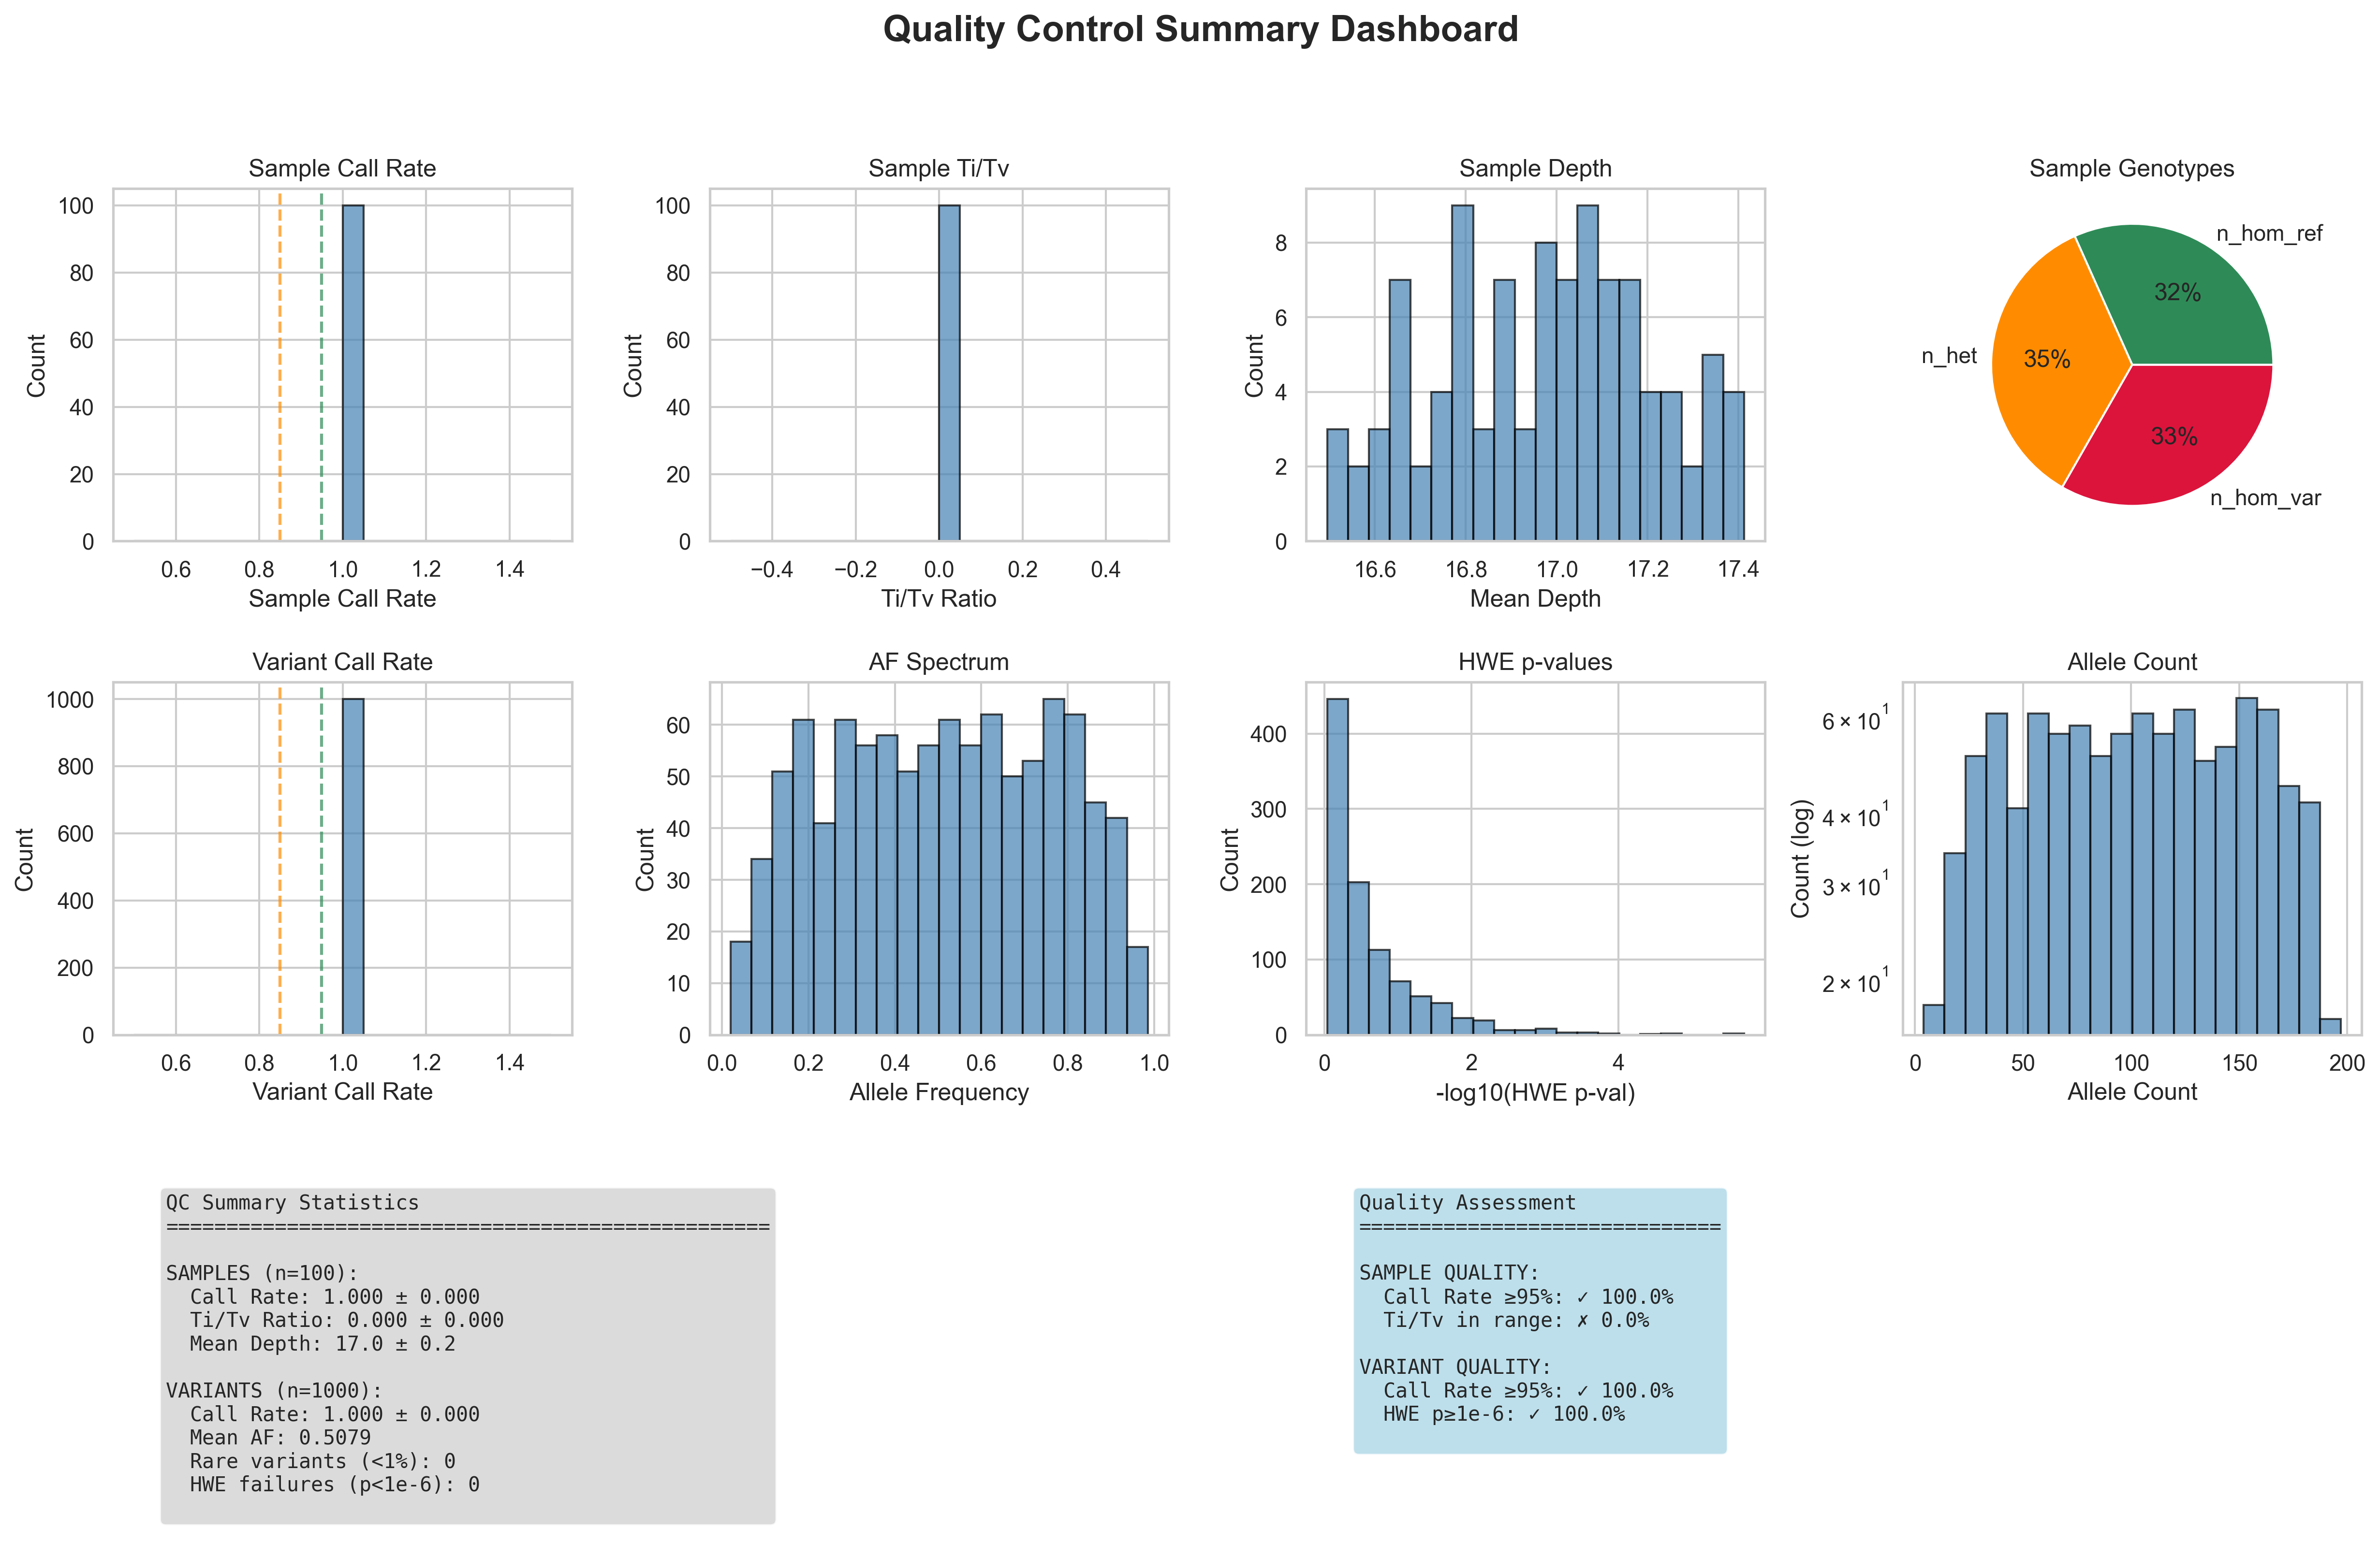
\includegraphics[width=\textwidth]{figures/fig_s5_qc_dashboard.png}
    \caption{QC Dashboard}
\end{subfigure}
\hfill
\begin{subfigure}[b]{0.48\textwidth}
    \centering
    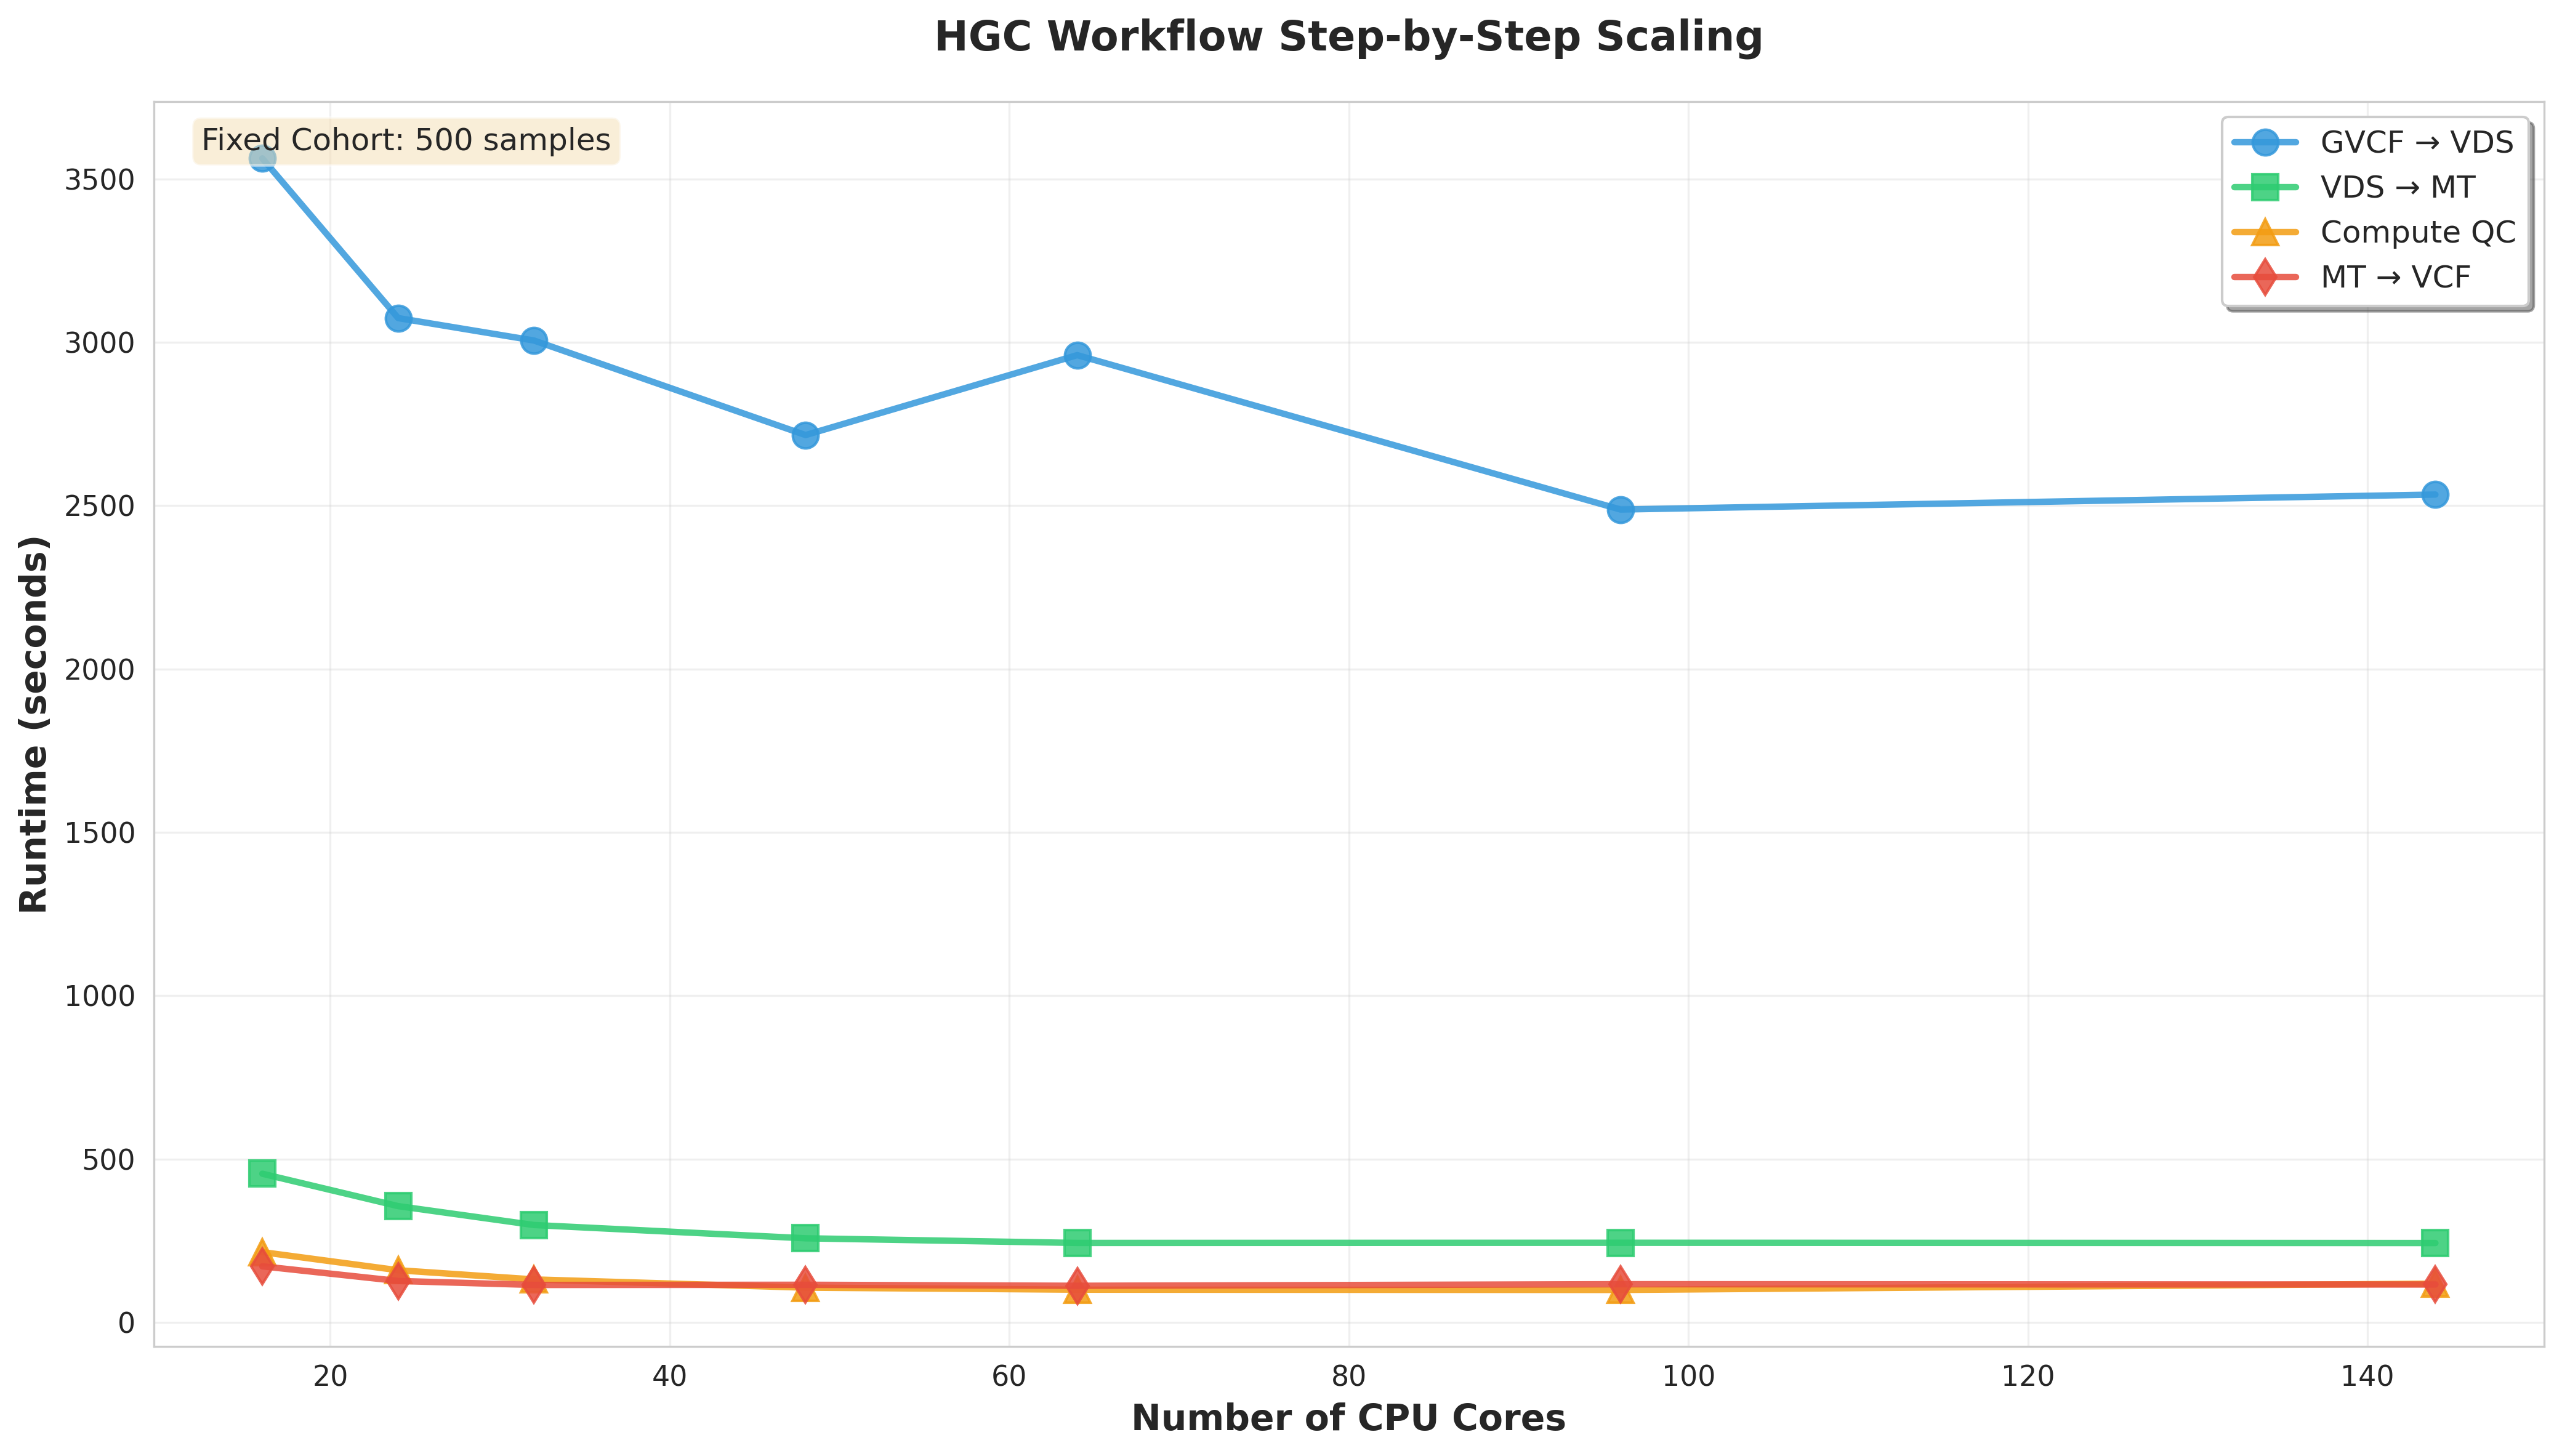
\includegraphics[width=\textwidth]{figures/fig_s6_cpu_scaling.png}
    \caption{CPU Scaling Performance}
\end{subfigure}
\caption{\textbf{Quality control and performance benchmarks.} (A) Example QC dashboard generated by hvantk showing sample-level metrics including call rate distribution, heterozygosity, Ti/Tv ratio, and variant-level statistics. (B) CPU scaling analysis showing execution time breakdown by workflow step, demonstrating efficient parallelization for large-scale analyses.}
\label{fig:results}
\end{figure}

%============================================================================
% EXAMPLE APPLICATION
%============================================================================
\section{Example Application}

The following workflow illustrates hvantk's integrated approach to variant annotation, score evaluation, and enrichment analysis:

\begin{lstlisting}[language=bash,caption={Example hvantk workflow for variant analysis}]
# Starting point: VDS from joint genotyping pipeline

# 1. Convert VDS to MatrixTable and compute QC
hvantk hgc vds2mt --vds cohort.vds --mt cohort.mt
hvantk hgc compute-qc --mt cohort.mt --generate-qc-report

# 2. Build multi-omics annotation tables
hvantk mktable clinvar --raw-input clinvar.vcf.bgz \
    --output-ht clinvar.ht --ref-genome GRCh38
hvantk mktable dbnsfp --raw-input dbNSFP.tsv.bgz \
    --output-ht dbnsfp.ht
hvantk mkmatrix gtex --output-mt gtex_expression.mt

# 3. Evaluate pathogenicity scores for candidate genes
hvantk psroc --genes MYBPC3,MYH7,TNNT2 \
    --clinvar-ht clinvar.ht --dbnsfp-ht dbnsfp.ht \
    --scores CADD_phred,REVEL_score --output-dir results/

# 4. Test burden in cardiomyopathy gene sets
hvantk enrichex burden --mt cohort.mt \
    --gene-sets cardiac_gene_sets.json \
    --phenotype affected --covariates PC1,PC2,PC3 \
    --af-threshold 0.001 --cadd-threshold 20
\end{lstlisting}

This workflow demonstrates hvantk's integrated capabilities: converting variant data to analysis-ready format with quality control, building multi-omics annotation tables, evaluating pathogenicity score performance for genes of interest, and testing whether rare damaging variants are enriched in disease-relevant gene sets.

%============================================================================
% CONCLUSION
%============================================================================
\section{Conclusion}

hvantk provides a scalable, Hail-native toolkit for variant annotation, multi-omics integration, and downstream enrichment analysis. By combining unified access to major genomic, transcriptomic, and proteomic resources with specialized analysis modules for pathogenicity score evaluation and gene set enrichment, hvantk bridges the gap between variant calling and biological interpretation. The toolkit seamlessly integrates with the VDS format for population-scale analyses while maintaining a user-friendly command-line interface. The modular, protocol-based architecture ensures extensibility as new annotation sources and analysis methods emerge.

%============================================================================
% ACKNOWLEDGEMENTS
%============================================================================
\section*{Acknowledgements}

We thank the developers of Hail and the VDS Combiner, and the maintainers of ClinVar, gnomAD, GTEx, and other public genomic resources for making their tools and data freely available.

\section*{Funding}

This work was supported by [funding sources to be added].

\section*{Conflict of Interest}

None declared.

%============================================================================
% REFERENCES
%============================================================================
\bibliographystyle{abbrvnat}
\bibliography{references}

\end{document}
